\documentclass[prl, twocolumn]{revtex4-2}
\usepackage{preamble}

\begin{document}
\title{GROUP 9 -- Restricted Boltzmann Machines to Learn Patterns in Biological Datasets}
\author{Davide Bacilieri}
\author{Lorenzo Barbiero}
\author{Guglielmo Bordin}
\author{Alessio Pitteri}
\date{\today}

\begin{abstract}
In the context of unsupervised learning, Restricted Boltzmann Machines
(RBMs) excel in the fields of pattern recognition and denoising; this leads
to application in various fields such as Information Theory or, in the case
of this paper, biological datasets.  In this paper, a RBM is built from an
Ising-like model, implementing a proper partition function, energy function
and log likelihood function that allows learning. Combining it with more
proper data analysis methods such as clever gradiend descents the
effectiveness of the framework is evaluated on plausible datasets for amino
acids recognition, both for known and unknown sequences.
\end{abstract}

\maketitle

\section{Introduction}
Restricted Boltzmann Machines belong to the class of energy-based
generative models. They are \emph{generative} in the sense that they
attempt to reproduce the underlying probability distribution that governs
the generation of the training data, in order to generate new samples that
could have been drawn from the same dataset \cite{Mehta2019}.

One use-case of this kind of models is in biology, with protein sequences
\cite{Tubiana2019, Tubiana2019_b}: RBMs can efficiently and reliably learn
complex and recurring patterns hidden in the sequences of amino acids.
Indeed, we worked on a very rudimentary implementation of this concept: our
dataset consisted of several short sequences of 1 and 0 bits, which could for 
example encode information about the alternation of polar and non-polar amino acids. 
The idea is to filter out the
noise and inconsistencies from the sequence, and grasp the underlying
pattern by having the RBM generate a “clean” sequence after training. Of
course, this has no pretence of actual resemblance to reality; it rather
serves as a proof of concept to show the capabilities of the learning
model.

The learning framework of RBMs strongly resembles many Ising-like models of
statistical physics. Taking the same equations, the problem is reframed as
the iterative learning of the parameters of a variational distribution that
should approximate the true distribution of the data.

Another thing that we borrow from physics is the concept of \emph{hidden
variables}. In Ising-like models, one usually performs a
Hubbard–Stratonovich transformation to avoid having to deal with the
complex quadratic interactions between spins, by shifting to the
description of a system of non-interacting spins immersed in a Gaussian
field \cite{Hubbard1959}. Similarly, in the context of Boltzmann learning,
we can simplify the complex relationships between the variables in the
training data by making them interact in a “controlled” manner with an
additional layer of fictitious variables. 

\section{Methods}
We will borrow the notation from the 2019 review on Machine Learning by
Mehta et al. \cite{Mehta2019}. Like we have said, Restricted Boltzmann
Machines are trained with the goal of best approximating a joint
probability distribution $p$ of the visible variables $\vec{v}$ and the
hidden variables $\vec{h}$, which, carrying on the analogy with statistical
physics models, is written as a Boltzmann distribution
\begin{equation}
    p(\vec{v}, \vec{h}) = \frac{e^{-E(\vec{v}, \vec{h})}}{Z},
\end{equation}
where the energy function $E(\vec{v}, \vec{h})$ takes the form
\begin{equation}
    E(\vec{v}, \vec{h}) = - \sum_{i = 1}^{N} a_i v_i - \sum_{\mu = 1}^{M}
    b_\mu h_\mu - \sum_{i = 1}^{N} \sum_{\mu = 1}^{M} W_{i \mu} v_i h_\mu.
    \label{eq:hamiltonian}
\end{equation}
We will refer to the variables $W_{i\mu}$ as \emph{weights}, and to the
coefficients $a_i$ and $b_\mu$ as \emph{biases}. These are the parameters
to learn, and we will collectively denote them with $\vec{\theta}$.

The actual training, that is, the iterative approximation of the true $p$
with a parametrized $p_{\vec{\theta}}$, is performed through the Maximum
Likelihood Estimation procedure. This involves the maximization – or
minimization of the negative – of the \emph{log-likelihood}
$\logL(\vec{\theta})$ of the model:
\begin{equation}
    \logL(\vec{\theta}) = -\expval{E(\vec{\theta})}_{\mathrm{data}} -
    \log(Z(\vec{\theta})).
\end{equation}
In practice, this translates to the application of (sto\-chas\-tic) gradient descent methods to the following set
of equations:
\begin{align}
    \pdiff{\logL(\vec{\theta})}{W_{i\mu}} &= \expval{v_i
    h_\mu}_{\mathrm{data}} - \expval{v_i h_\mu}_{\mathrm{model}},
    \label{eq:dL_dW} \\
    \pdiff{\logL(\vec{\theta})}{a_i} &= \expval{v_i}_{\mathrm{data}} -
    \expval{v_i}_{\mathrm{model}}, \label{eq:dL_da} \\
    \pdiff{\logL(\vec{\theta})}{b_\mu} &= \expval{h_\mu}_{\mathrm{data}} -
    \expval{h_\mu}_{\mathrm{model}}. \label{eq:dL_db}
\end{align}
Here the expectation values with respect to the data are the empirical
averages on the training samples, while the expectation values with respect
to the model need to be estimated by drawing samples from the parametrized
distribution $p_{\vec{\theta}}$.

Going back to the problem at hand the employed RBM features two hidden units and carries out gradient descent in mini-batches of 500 samples, with the possibility to use either \emph{RMSProp} or \emph{ADAM} for the minimization. In our case, the gradient descent procedure was conducted with the \emph{ADAM} algorithm (as described in
\cite{Mehta2019}). 

To calculate the expectation values in
Eqs.~\eqref{eq:dL_dW}–\eqref{eq:dL_db}, we performed three steps of block
Gibbs sampling (so, a \emph{three-step Contrastive Divergence}), each step
being a forward sample from the visible layer to the hidden layer, plus a
backward sample in the opposite direction.

We should now specify that our training data consisted of many sequences of
one-hot encoded blocks of units of length $B$. These blocks were interpreted as
encodings for the different amino acids chaining to form a “protein”. So,
while the hidden layer posed no sampling problems – the $h_\mu$s are
simple binary variables – the backward sample on the visible layer required
some special attention due to the one-hot encoding.

Let us define the possible values of each data block in $\vec{v}$ as
$\vec{v}^{(k)}$, with $k = 1, \dots, 6$ denoting the position of the
positive bit. During the backward sampling, we have to clamp the variables
in the visible layer to every possible configuration and compute their
respective probability. Therefore, a given block has $B$ different
probabilities associated to it:
\begin{equation}
    p(\vec{v}^{(k)} \given \vec{h}) = \frac{1}{Z} \exp\left[a_k + \sum_{\mu
    = 1}^{M} (b_\mu + W_{k\mu}) h_\mu \right].
    \label{eq:p-vk-given-h}
\end{equation}
The partition function $Z$ is the sium of the $B$ probabilities, so the term
with $\vec{b}$ cancels out. In practice, for each block of $B$ units in
$\vec{v}$, we computed the cumulative probabilities $C_k$ as $\tilde{C}_k /
\tilde{C}_B$ with
\begin{equation}
    \tilde{C}_k = \sum_{i = 1}^{k} \exp\left(a_i + \sum_{\mu = 1}^{M}
    W_{i\mu} h_\mu\right)
    \label{eq:C-tilde}
\end{equation}
Then, we generated a random number $r$, chose $\ell$ such that
$C_{\ell-1}<r<C_\ell$, and replaced the block with $\vec{v}^{(\ell)}$. 

We also explored the possibility to work with “spins” instead of bits, i.e.
$+1$/$-1$ binary variables. Eq.~\eqref{eq:p-vk-given-h} has to be reworked a
bit, giving
\begin{equation}
    p(\vec{v}^{(k)} \given \vec{h}) = \frac{1}{Z'}
    \exp\Biggl[
        - \sum_{j = 1}^{B} (-1)^{\delta_{jk}} \Biggl(a_j + \sum_{\mu =
        1}^{M} W_{j\mu} h_\mu\Biggr)
    \Biggr],
    \label{eq:p-vk-given-h-spins}
\end{equation}
where $Z'$ is the partition function without the terms with $\vec{b}$ that
cancel out. We can use a similar expression as Eq.~\eqref{eq:C-tilde} but
with a factor of $2$ multiplying the argument of the exponentials. The reason
for this becomes clear if we factor out
\begin{equation}
    \exp\Biggl[-\sum_{j = 1}^{B} \Biggl(a_j + \sum_{\mu = 1}^{M} W_{j\mu}
    h_\mu\Biggr)\Biggr]
\end{equation}
from Eq.~\eqref{eq:p-vk-given-h-spins}.

Although the $+1$/$-1$ representation has undoubtedly a nice connection to 
Physics notation, the $1$/$0$ version turned out to be more computationally 
efficient and conceptually easier to implement. So, in the end we opted for the 
latter.

As regards the calculation of the partition function $Z$ that enters the expression
of the log-likelihood, the $0$/$1$ format permits the following simplification:
\begin{equation}
\begin{split}
    Z&=\sum_{\{\vec{v}, \vec{h}\}} e^{-E_{\vec{\theta}}(\vec{v}, \vec{h})}\\
    &=\sum_{\{\vec{h}\}} e^{B\vec{b}\cdot\vec{h}} \prod_{j=0}^{N_B} ~ \sum_{k=j}^{j+B-1} e^{a_k+W_{k\mu}h_\mu},
    \end{split}
\end{equation}
where the sums on $\{\vec{v}, \vec{h}\}$ and $\{\vec{h}\}$ denote the sum over all possible
configurations of positive and negative bits.

Before moving on to the results discussion, we should mention that we
implemented the Adversarial Accuracy Indicator (AAI) from \cite{Yale2020} to
provide a meaningful rating for our trained model. The task of finding accuracy 
indicators in the context of generative learning has no definitive solution, 
unlike in supervised learning. With AAI, the similarity between the original 
dataset and a generated one is gauged by counting how many times a given data 
point’s nearest neighbour belongs to the same set and how many times it belongs 
to the other; if indeed the sets came from the same probability distribution, 
the ratio of nearest neighbours of the same type to the total number of samples should approach $1 / 2$. 
The distance we used to choose the nearest points is a Manhattan-like distance in L dimensions, consisting in counting how many bits are different between two sequences. 
We perform this procedure for the whole dataset divided in mini-batches composed of only 10 sequences because there are high chances that in a larger dataset many samples will find an exact copy of themselves.


\section{Results}
We had two datasets at our disposal: one with one-hot encoded blocks of 4 bits and another with 6-bit blocks. The pattern in the 4-bit dataset was known a priori, unlike the pattern in the 6-bit data. Therefore, the plan was to use the first dataset to evaluate the model’s performance. If the result was satisfactory, we would have proceeded to analyse the unknown dataset.

The training with the 4-bit dataset went smoothly, and the model correctly guessed the schema.
The pattern to learn was the alternance of two kinds of “amino acids”. One of the amino acids was
identified by either of the two one-hot blocks with the positive bit in the first two positions, 
while the other two blocks identified the other amino acid. To preserve the physical analogy, we 
can classify the first type as a general polar amino acid and the second type as a non-polar
amino-acid. As in the real world, a polar amino acid comes after a non-polar one in a linear sequence.

\begin{figure}
    \centering
    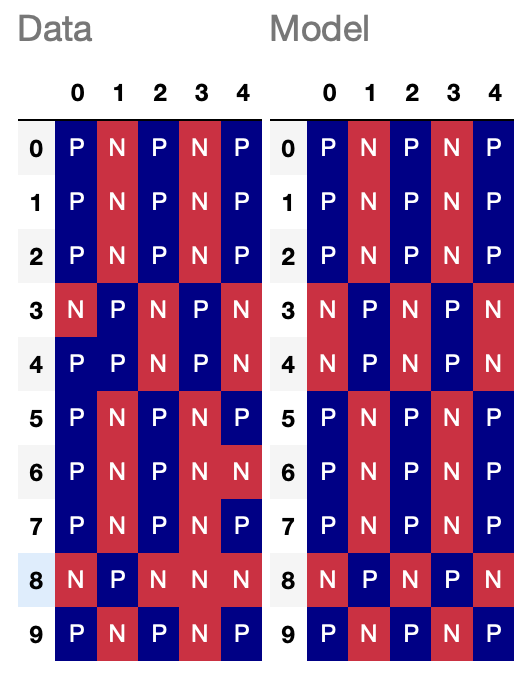
\includegraphics[width=0.6\linewidth]{plots/PN4bits.png}
    \caption{Excerpt from the original dataset with 4-bit blocks next to one generated
    by the model. \emph{N} stands for \emph{non-polar}, \emph{P} for \emph{polar}.}
    \label{fig:4-bit-PNP}
\end{figure}

In \figref{fig:4-bit-PNP}, you can see a comparison between a portion of the original dataset and a generated one. The original dataset has some noise that disrupts the polar/non-polar alternation in various places, while the generated sample corrects the
imperfections and returns correct sequences in every line. The denoised sequences are computed using the biases and weights from the last epoch in training, with a single divergent step.

We also introduced a parameter $\beta$ to rescale the energy and simulate a decrease in temperature, reducing the 
stochasticity in the generation. This is analogous to the temperature in an Ising-like system; in fact, 
the Hamiltonian \eqref{eq:hamiltonian} can be mapped to that of a Hopfield model \cite{Mehta2019} (with the important distinction that the hidden layer is binary instead of Gaussian). We know then that perfect pattern retrieval happens only when the temperature is low enough.



6 BITS 1 HOE

The weights heatmap suggests an underlying pattern: we can guess that the blocks are of two different types if $\vec{v}^{(k)}$ with $k=1,2,3$ or $k=4,5,6$. Once the denoising procedure is completed, the unknown distribution of the blocks seems to be an alternation of same-type block pairs. We maintain the notation with N and P, but they lose the meaning of polar and nonpolar amino acids.
%heatmap 



\bibliography{biblio}
\end{document}
